\section{Esercizio 15}

\begin{itemize}
\item Ascisse equidistanti
\lstinputlisting[language=Matlab]{CodiceMatlab/Esercizio15-19/ascisseEquidistanti.m}
\item Ascisse di Chebyshev
\lstinputlisting[language=Matlab]{CodiceMatlab/Esercizio15-19/chebyshev.m}
\item Utilizzando il polinomio di newton
\lstinputlisting[language=Matlab]{CodiceMatlab/Esercizio15-19/scriptEs15.m}
\end{itemize}

\newpage
\begin{figure}[h!]
    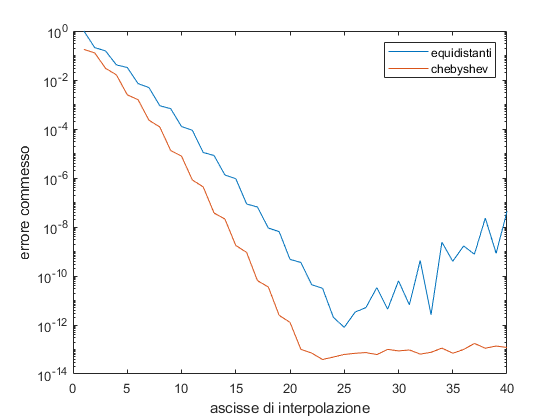
\includegraphics[scale=0.8]{CodiceMatlab/Esercizio15-19/graficoEs15.png}
    \caption{Grafico esercizio 15 con newton}
    \label{fig:es15}    
\end{figure}


\begin{figure}[h!]
    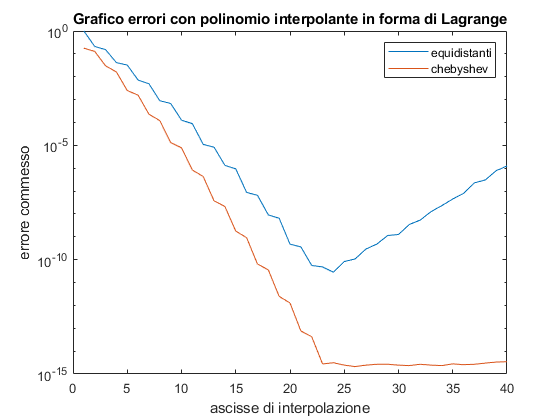
\includegraphics[scale=0.8]{CodiceMatlab/Esercizio15-19/graficoEs15Lagrange.png}
    \caption{Grafico esercizio 15 con Lagrange}
    \label{fig:es15}    
\end{figure}
Possiamo notare dal grafico 1  che l'errore nel caso delle ascisse di chebyshev è costantemente minore rispetto a quello delle ascisse equidistanti. Dopo n = 23  il grafico dell'errore commesso utilizzando le ascisse di chebyshev presenta un andamento costante. Per le ascisse equidistanti ( utilizzando i metodo di newton ) invece, l'errore raggiunge il valore minimo a n =25 , e  in seguito inizia a salire con un andamento non costante.\\
Possiamo notare che il grafico 2 è molto simile a quello precedente per quanto riguarda le ascisse di chebyshev. Mentre per le ascisse equidistanti, l'errore dopo aver raggiunto il suo valore minimo non presenta l'andamento a "zig zag".\\
Al crescere del numero delle ascisse di interpolazione l'errore commesso scegliendo le ascisse di chebyshev rimane più o meno costante in entrambi i casi. Questo è dovuto al fatto che la costante di Lebesgue equivale a circa $\frac{2}{\pi}\log{n}$, e risulta quindi avere una crescita ottimale, mentre per le ascisse equidistanti invece si ha una crescita esponenziale al crescere di n.
